\chapter{Supervisory Interface} \label{ch:interface}

\section{Current Implementation}

The supervisory layer for the prototype is a Python command-line interface (CLI) running on a laptop, communicating with the STM32F303 microcontroller over UART via USB. This interface was used for all testing and demonstration described in Chapter~13.

The CLI accepts human-readable commands and serialises them into JSON packets for transmission to the STM32. The supported command set includes:

\begin{itemize}
    \item \textbf{Absolute move:} Specify target positions for one or more axes in millimetres or degrees. The CLI converts physical distances to step counts using the electronic gear ratio and transmission parameters established in Chapters~6 and~9, and transmits the resulting step/direction commands.
    \item \textbf{WASD teleoperation:} Real-time manual control of the X and Y axes via keyboard input, used during the showcase demonstrations for pick-and-move operations.
    \item \textbf{Homing:} Triggers the homing routine described in Section~9.4 on the specified axes.
    \item \textbf{Pin remapping:} Allows reassignment of step and direction GPIO pins at runtime, enabling hardware debugging without reflashing firmware.
    \item \textbf{Parameter tuning:} Adjusts speed, acceleration, and motion profile parameters transmitted to the STM32.
\end{itemize}

The STM32 echoes its internal state (current step counts, direction flags, and axis status) back to the CLI as JSON, providing confirmation that commands were received and executed. Figure~\ref{fig:gantry_cli} shows a representative session.

\begin{figure}[H]
    \centering
    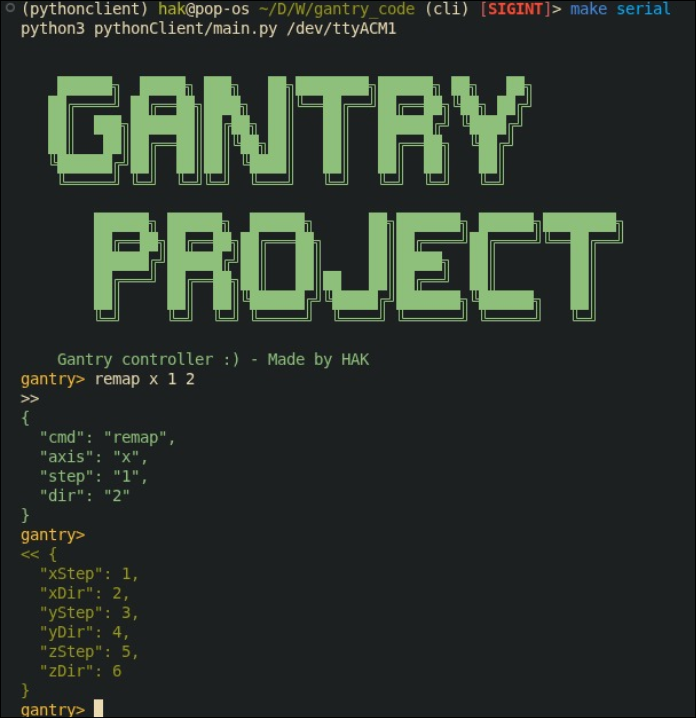
\includegraphics[width=0.85\linewidth]{figures/gantry_project_cli.png}
    \caption{The gantry CLI showing a pin remapping command and the STM32's state echo.}
    \label{fig:gantry_cli}
\end{figure}

This interface is sufficient for development, testing, and demonstration, but is not suitable for production deployment. Factory line operators cannot be expected to interact with a terminal, and the CLI provides no automated sequencing --- every move must be commanded manually.

\section{Planned Deployment Architecture}

For production deployment, the intended architecture replaces the CLI with a ROS2-based supervisory system running on an industrial PC. Table~\ref{tab:ros2_nodes} outlines the planned node structure, which was designed during the project but not implemented on the prototype due to the priority placed on validating the lower-level subsystems first.

\begin{table}[H]
    \centering
    \caption{Planned ROS2 node architecture for production deployment.}
    \label{tab:ros2_nodes}
    \renewcommand{\arraystretch}{1.2}
    \small
    \begin{tabular}{@{}l l p{3cm} p{4.5cm}@{}}
        \toprule
        \textbf{Node} & \textbf{Publishes} & \textbf{Subscribes} & \textbf{Role} \\
        \midrule
        \texttt{camera\_node} & \texttt{/image\_raw} & --- & Streams frames from the AR0234 camera. \\
        \texttt{vision\_node} & \texttt{/target\_pose} & \texttt{/image\_raw} & Runs the detection and pose estimation pipeline (Chapter~10). \\
        \texttt{planner\_node} & \texttt{/trajectory} & \texttt{/target\_pose} & Computes pick-and-place trajectories from current and target poses. \\
        \texttt{controller\_node} & \texttt{/joint\_cmds} & \texttt{/trajectory}, \texttt{/joint\_states} & Tracks the planned trajectory; issues step commands to the STM32. \\
        \texttt{hw\_interface} & \texttt{/joint\_states} & \texttt{/joint\_cmds} & Serial bridge to the STM32; relays commands and reads encoder feedback. \\
        \texttt{vacuum\_node} & --- & \texttt{/vacuum\_cmd} & Toggles the solenoid valve via GPIO. \\
        \texttt{supervisor\_node} & \texttt{/vacuum\_cmd} & \texttt{/target\_pose}, \texttt{/joint\_states} & Finite state machine: Idle $\rightarrow$ Detect $\rightarrow$ Align $\rightarrow$ Pick $\rightarrow$ Transfer $\rightarrow$ Place. \\
        \bottomrule
    \end{tabular}
\end{table}

The key addition over the current CLI is the \texttt{supervisor\_node}, which would implement the finite state machine that automates the full pick-and-place cycle without manual intervention. This node was validated in the PyBullet simulation (Chapter~\ref{ch:prototyping}) but has not been deployed on physical hardware. Its implementation, along with the development of an operator HMI to replace the CLI, is recommended as a near-term commissioning step in Section~\ref{sec:near_term}.